\section{Specific Requirements}
(R1.1) The system allows students that don't have an account to sign up for the first time on the platform.  \\
(R1.2) The system allows students that already have an account to log in the platform.\\
(R1.3) The system notifies all students that have an account on the platform every time a new tournament is created.\\
(R1.4) The system shows to a student the list of tournaments available on the platform, including closed tournament, the ones the student is already subscribed to and the ones s/he can subscribe to. \\
(R1.5) The system allows students to join the tournaments they’re interested in, by the end of the registration deadlines set for the tournaments.  \\
(R1.6) The system notifies all students subscribed to a tournament every time a new battle within that tournament is published.  \\
 (R1.7) The system allows students subscribed to a tournament to join battle(s) within that tournament, by the end of the registration deadline set for the battle(s). \\
 (R1.8) The system allows students subscribed to a tournament to join a battle of the tournament either on their own or creating teams with other students.  \\
 (R1.10) The system sends the link of the GitHub repository dedicated to a battle to all the students subscribed to that battle. \\
 (R1.11) The system notifies all students participating in a battle when the battle terminates and the final ranking of teams is available on the platform.  \\
 (R1.12) The system notifies all students subscribed to a tournament when the tournament is closed by the educator who created it.
 (R1.13) The system creates a new GitHub repository dedicated to a battle when the registration deadline for that battle passes. \\
(R1.14) The system accepts notifications from GitHub in order to know when a new commit is performed by a student in any GitHub repository dedicated to an ongoing battle.  \\
(R1.15) The system pulls from the GitHub repositories of ongoing battles the new students' code solutions, every time it receives a notification from GitHub of a new commit in those repositories.  \\
(R1.16) The system recalculates and then publishes the new score of a team's solution every time it receives a notification from GitHub of a new commit performed by a member of the team.  \\
(R2.1) The system allows educators that don’t have an account to sign up for the first time on the platform. \\
(R2.2) The system allows educators that already have an account to log in the platform. \\
(R2.3) The system allows educators to create new tournaments.  \\
(R2.4) The system allows educators to set a registration deadline for the tournament(s) they want to create  \\
(R2.6) The system allows the educator that created a tournament to grant the permission of publishing battles within his/her tournament to other educators on the platform. \\
(R2.7) The system allows educators to create new battle(s) in the tournaments they have the permissions to do so \\
(R2.8) The system allows educators to upload on the platform the textual description of a battle they want to create.  \\
(R2.9) The system allows educators to set a minimum and maximum number of members for each team of students participating in the battle they want to create  \\
(R2.10) The system allows educators to declare whether to require a consolidation stage or not at the end of the battle they want to create.  \\
(R2.11) The system allows educators to specify what parameters of evaluation (reliability, security...) should be used by the system in order to compute the scores of the students' code solutions through static analysis external tools.  \\
(R2.12) The system allows educators to set a registration deadline for the battle they want to create.  \\
(R2.13) The system allows educators to set a submission deadline for the battle they want to create.  \\
(R2.14) The system doesn't take into account any new code solution for a battle after the submission deadline of that battle.  \\
(R2.15) After the submission deadline of a battle and only if a consolidation stage had been requested by the educator at battle creation time, the system sets a time frame for the educator that created the battle to allow him/her to assign personal scores to the students’ code solutions.  \\
(R2.16) The system takes into account the personal scores assigned by the educator during the consolidation stage of a battle only if the educator assigned a score to all teams within the imposed time frame. \\
(R2.17) At the end of a battle and after the consolidation stage (if requested), the system automatically calculates and publishes the final rank of all teams that participated in that battle.  \\
(R2.18) When a tournament is closed, the system automatically publishes the rank of all students that participated in the tournament. \\
(R3.1) The system allows students subscribed to the same tournament to invite each other in order to join battles as a team, respecting the minimum and maximum number of students permitted for a team in the battle. \\
(R3.2) The system calculates and then publishes the score assigned to a new code solution of a team in a battle, every time GitHub notifies the platform of a new commit performed by a member of such team. \\
(R3.3) The system constantly keeps updated the total ranking of teams for a battle, which evolves based on the new code solutions that are uploaded by students on the GitHub repository. \\
(R3.4) The system calculates and publishes the final ranking of teams when a battle ends. \\
(R3.5) The system allows only the educators and students involved in a battle to see the partial or final ranking of teams for that battle. \\
(R3.6) The system automatically calculates and keeps updated the total ranking of students subscribed to a tournament, based on the scores each student received in the battles he participated in. \\
(R3.7) The system allows all users on the platform to see the partial or final rankings of tournaments. \\
(R3.8)  The system allows educators to define customary badges (rewards) for the students participating in their tournaments, at tournament creation time. \\
(R3.9) The system assigns badges (rewards) to students that participated in a tournament when the tournament is closed by the educator that created it. \\
(R3.10) The system allows all users on the platform to search for the personal profile of a student and see the corresponding page. \\
(R3.11) The system allows all users on the platform to see the list of badges owned by a student for the tournaments s/he participated in. \\
\subsection{External Interface Requirements}
\subsubsection{User Interface}
This section is dedicated to the illustration of some mockups of the most relevant graphical user interfaces that \app uses to interact with external users (educators and students). 
The aim of these representations is to specify the logical characteristics of the presented interfaces as well as introducing some guidelines on the style and look that the final product will have. This information can be used in order to shape the design of the \app platform in more advanced stages of the development.
 
\vspace{1cm}

\begin{minipage}{\linewidth}
	\textbf{Log In Interface}
  \begin{center}
  \includegraphics[page=1,width=0.7\linewidth,keepaspectratio]{3Specific_Requirements/res/UI_Mockup}

  \end{center}
    Log In Interface for both Educators and Students, who can access \app through their GitHub account by clicking on the button "Login Through GitHub"
\end{minipage}

\vspace{1cm}

\begin{minipage}{\linewidth}
	\textbf{Home Page Student}
	\begin{center}
		\includegraphics[page=2,width=0.7\linewidth,keepaspectratio]{3Specific_Requirements/res/UI_Mockup}
		
	\end{center}
	Home page for a student, in which it is possible to:
	\begin{itemize}
		\item See personal profile of the student, with a customary image.
		\item See the list of badges earned by the student in tournaments s/he participated in.
		\item Ask for the list of tournaments the student is subscribed to.
		\item Subscribe to a new tournament with the "Join Tournament" button.
		\item Search for a user on the platform (with the magnifying glass in the top right corner). 
	\end{itemize}
\end{minipage}

\vspace{1cm}

\begin{minipage}{\linewidth}
	\textbf{Home Page Educator}
	\begin{center}
		\includegraphics[page=3,width=0.7\linewidth,keepaspectratio]{3Specific_Requirements/res/UI_Mockup}
		
	\end{center}
	Home page for an educator, in which it is possible to:
	\begin{itemize}
		\item See personal profile of the educator, with a customary image.
		\item Ask for the list of tournaments the educator created (or has permissions to publish battles in), with the "My Tournaments" button.
		\item Create a new battle with the "New Battle" button. 
		\item Create a new tournament with the "New Tournament" button.
		\item Search for a user on the platform (with the magnifying glass in the top right corner). 
	\end{itemize}
\end{minipage}

\vspace{1cm}

\begin{minipage}{\linewidth}
	\textbf{Tournament Creation Form}
	\begin{center}
		\includegraphics[page=4,width=0.7\linewidth,keepaspectratio]{3Specific_Requirements/res/UI_Mockup}
		
	\end{center}
 	This interface pops up when the educator clicks on "New Tournament" from the home page. Thanks to this form, all relevant parameters for the creation of a tournament can be set.

\end{minipage}

\vspace{1cm}

\begin{minipage}{\linewidth}
	\textbf{Tournament Creation Form}
	\begin{center}
		\includegraphics[page=5,width=0.7\linewidth,keepaspectratio]{3Specific_Requirements/res/UI_Mockup}
		
	\end{center}
	This interface pops up when the educator clicks on "New Tournament" from the home page. Thanks to this form, all relevant parameters for the creation of a tournament can be set.
	
\end{minipage}
\subsubsection{Hardware Interfaces}
The system offers the services described in section 2 via different hardware interfaces as CodeKataBattle services are provided via a web page and via a mobile application.
To access the service offered by the system both kind of users are required to have either a device with an internet connection, to access the web page, or the mobile application.
Students are also required to have access to a computer with internet connection to be able to access the GitHub page containing the material for the battle and to be able to manage their GithHub projects.

\subsubsection{Software Interfaces}
The system requires some software interfaces in order to provide its services. Below are reported the most significant:
\begin{itemize}
    \item GitHub API Integration : The system communicates with external APIs to allow the creation of GithHub repositories for each battle
\end{itemize}
\subsection{Functional Requirements}
\subsubsection{Use Case Diagrams}

\includegraphics*[width=18cm,keepaspectratio]{UseCaseDiagram1}
\vspace*{3cm}
\includegraphics*[width=12cm,keepaspectratio]{UseCaseDiagram2}
\subsubsection{UseCases}

\renewcommand{\arraystretch}{1.9}

	

    \begin{longtable}{|p{3cm}p{14cm}|}
    \multicolumn{2}{l}{\textbf{[UC1] - EducatorLogIn} }\\
        \hline 
         Name & EducatorLogIn \\
        \hline 
        Actors & Educator, GitHub. \\
        \hline
        Entry Condition & Educator has opened \app on his/her laptop. \\
        \hline
        Event Flow &  
        	1 - \app shows the log in interface with the button to sign in with a GitHub account.

        	2 - Educator clicks on the button to sign in using his/her GitHub account.

        	3 - \app redirects the educator to the GitHub login page.
        	
        	4 - Educator inserts his/her GitHub credentials and confirms.\\
        \hline
        Exit Condition & \app shows the initial (home) page of the application for an educator.  \\
        \hline
        Exceptions & 
        	1 - Educator inserts wrong credentials to access his/her GitHub account: the GitHub authentication page will return an error to the educator, asking him/her to retry.\\
        \hline
      
    \end{longtable}
      
	
	
	\begin{longtable}{|p{3cm}p{14cm}|}
		\multicolumn{2}{l}{\textbf{[UC2] - StudentLogIn}}\\
		\hline
		Name & StudentLogIn \\
		\hline
		Actors & Student, GitHub. \\
		\hline
		Entry Condition & Student has opened \app on his/her laptop. \\
		\hline
		Event Flow &  
		
		1 - \app shows the log in interface with the button to sign in with a GitHub account.
		
		2 - Student clicks on the button to sign in using his/her GitHub account.
		
		3 - \app redirects the student to the GitHub login page.
		
		4 - Student inserts his/her GitHub credentials and confirms.
		\\
		\hline
		Exit Condition & \app shows the initial (home) page of the application for an student.  \\
		\hline
		Exceptions & 
		1 - Student inserts wrong credentials to access his/her GitHub account: the GitHub authentication page will return an error to the student, asking him/her to retry.\\
		\hline
    
    \end{longtable}
    
    
      \begin{longtable}{|p{3cm}p{14cm}|}
      	\multicolumn{2}{l}{\textbf{[UC3] - CreateTournament}}\\
        \hline
         Name & CreateTournament \\
        \hline
        Actors & Educator, Student. \\
        \hline
        Entry Condition & Educator is logged in the \app platform.  \\
        \hline
        Event Flow &  
        	1 - Educator clicks on the button to create a new tournament.
        	 
        	2 - \app shows the form to fill with the information for the tournament to be created.
        	
        	3 - Educator types in the name of the tournament.
        	
        	4 - Educator writes down a description of the tournament.
        	
        	5 - Educator defines the registration deadline by which students are asked to register for the tournament if interested.
        	
        	6 - Educator defines the badges (rewards) to be assigned to students at the end of the tournament based on some customary achievements.
        	
        	7 - Educator confirms the information filled in the form.
        	
        	8 - \app shows the initial page of the tournament to the educator.
        	
        	8 - \app sends a notification to all the students on the platform to inform them of the new tournament available.\\
      
        
        \hline
        Exit Condition & The new tournament is added to the list of tournaments created by the educator and all users on the platform can see the new tournament. \\
        \hline
        Exceptions &
        1 - The registration deadline set by the educator is on the same day or before the day in which the educator is trying to create the new tournament: the system does not allow the educator to confirm the creation of the tournament and reports an error message.
        
        2 - Educator confirms the form to create the new tournament leaving some mandatory information unspecified: in this case \app will return an error message to the educator stating that some information is missing and the tournament cannot be created.\\
        \hline
        Special Requirements & Mandatory data in the tournament creation form is composed of name and registration deadline of the tournament.
        \\
        \hline
      
    \end{longtable}

    
      \begin{longtable}{|p{3cm}p{14cm}|}
      	\multicolumn{2}{l}{ \textbf{[UC4] - CreateBattle}}\\
        \hline
         Name & CreateBattle \\
        \hline
        Actors & Educator, Student. \\
        \hline
        Entry Condition & Educator is logged in the \app platform and has the permissions to publish a battle in the tournament which the battle will reside in. S/he has already written the build automation scripts and test cases for the battle to be created. \\
        \hline
        Event Flow & 
        	1 - Educator clicks on the button to create a new battle from the home page of \app.
        	
        	2 - \app displays the entire list of tournaments in which the educator has permissions to publish battles.
        	
        	3 - Educator selects the tournament in which s/he wants to create the new battle.
        	
        	4 - \app shows the form to fill in with all the relevant data associated with the battle.
        	
        	5 - Educator types in the name of the battle.
        	
        	6 - Educator writes down the textual description of the battle.
        	
        	7 - Educator uploads the build automation scripts related to the battle.
        	
        	8 - Educator uploads the test cases related to the battle.
        	
        	9 - Educator sets the registration deadline for the battle, by which students are asked to join if interested.
        	
        	10 - Educator sets the submission deadline for the battle, after which \app stops accepting additional solutions to the battle.
        	
        	11 - Educator sets the minimum and maximum number of students allowed per team.
        	
        	12 - Educator selects the aspects on which \app automatically evaluates the students' code solutions, leveraging an external static analysis tool. For instance maintainability, security...
        	
        	13 - Educator specifies whether a consolidation stage for personal evaluation of the students' code solutions is required at the end of the battle.
        	
        	14 - Educator clicks on the button to confirm the data inserted in the form.
        	
        	15 - \app shows the educator the presentation page of the newly created battle.
        	
        	16 - \app sends a notification to all the students subscribed to the tournament in which the battle has been created, informing them of the new battle available.
        \\
        \hline
        Exit Condition & The new battle is added on the list of battles created by the educator and students are able to see this new battle in the tournament in which it resides. \\
        \hline
        Exceptions & 
        
        1 - The registration deadline set by the educator is on the same day or before the day in which the educator is trying to create the new battle: the system does not allow the educator to confirm the creation of the battle and reports an error message.
        
       	2 - The submission deadline set by the educator is on the same day or before the day of the registration deadline: the system does not allow the educator to confirm the creation of the tournament and reports an error message.
        
        3 - Educator confirms the creation of the battle without uploading either the build automation scripts or the test cases for the battle: the system doesn't create any new battle and reports an error message to the educator stating the reason why the battle cannot be instantiated.
        
        4 - Educator confirms the creation of the battle without specifying some mandatory information for the battle: the system doesn't create any new battle and reports an error message to the educator stating the reason why the battle cannot be instantiated.\\
        \hline
        Special Requirements & Mandatory data in the battle form include the battle's name, the textual description of the problem to be solved, the registration and submission deadlines, the minimum and maximum number of students per team.\\
         \hline
      
    \end{longtable}
      
     \begin{longtable}{|p{3cm}p{14cm}|}
     	\multicolumn{2}{l}{\textbf{[UC5] - GrantPermissions}}\\
        \hline
        Name & GrantPermissions \\
        \hline
        Actors & Educator. \\
        \hline
        Entry Condition & Educator A is logged in the system. Educator A created a tournament on the platform. \\
        \hline
        Event Flow &  
        1 - Educator A selects from the home page of \app the button to visualize the list the tournaments that s/he created.
        
        2 - \app displays the list of tournaments created by educator A.
        
        3 - Educator A clicks on the tournament in which s/he wants to grant permissions to educator B.
        
        4 - \app opens the description page of the selected tournament.
        
        5 - Educator A clicks on the button to grant the permissions to publish battles to another educator in the tournament.
        
        6 - \app displays an interface to search for an educator by username.
        
        7 - Educator A types in educator B's username, finds him/her and confirms the choice.
        
        8 - \app sends a request to educator B to inform him/her of the possibility to publish battles in A's tournament.
        
        9 - Educator B accepts the request.
        \\
        \hline
        Exit Condition & The system adds the tournament to the list of tournaments in which educator B has permissions to publish battles.\\
        \hline
        Exceptions & 
        1 - Educator A tries to grant publishing permissions to educator B who already had permissions on that tournament: \app doesn't modify anything on B's account and reports to A that B already had publishing permissions on that tournament.
        
        2 - Educator A tries to grant publishing permissions to educator B on a closed tournament: \app doesn't modify anything on B's account and reports to A the tournament is already terminated.
        \\
        \hline
      
    \end{longtable}

    
      \begin{longtable}{|p{3cm}p{14cm}|}
      	\multicolumn{2}{l}{\textbf{[UC6] - SubscribeToTournament}}\\
        \hline
        Name & SubscribeToTournament \\
        \hline
        Actors & Student. \\
        \hline
        Entry Condition & The student is logged in the system.\\
        \hline
        Event Flow &  
        1 - \app displays the list of available tournaments on the platform in the home page.
        
        2 - Student browses the list of available tournaments and reads some of their descriptions to get an idea on them.
        
        3 - Student clicks on the tournament wants to subscribe to.
        
        4 - \app shows the home page of the selected tournament.
        
        5 - Student clicks on the button to subscribe to the tournament and confirms his choice.
        \\
        \hline
        Exit Condition & The system adds the tournament to the list of tournaments the student is subscribed to. \\
        \hline
        Exceptions & 
        1 - Student tries to subscribe to a tournament whose registration deadline has already passed: \app reports an error message to the student stating that it is not possible to carry out the operation.
        \\
        \hline
    \end{longtable}

   

      
     \begin{longtable}{|p{3cm}p{14cm}|}
     	\multicolumn{2}{l}{\textbf{[UC7] - JoinBattleAlone}}\\
        \hline
        Name & JoinBattleAlone \\
        \hline
        Actors & Student. \\
        \hline
        Entry Condition & The student is logged in the platform and is subscribed to the tournament in which the battle s/he wants to join resides.\\
        \hline
        Event Flow &  
        1 - Student opens the list of tournaments s/he's subscribed to from the home page of \app.
        
        2 - \app displays the list of tournaments the student is subscribed to.

        3 - Student clicks on the tournament in which the battle s/he wants to join resides.

        4 - \app shows the home page of the selected tournament.
        
        5 - Student selects the battle s/he wants to join and clicks on it.

        5 - \app shows the description page of the selected battle with the button to join it.
        
        6 - Student clicks the button to join the battle.
        
        7 - \app shows the interface for joining a battle, in which it is possible to decide whether to participate as a single player or with other students as a team.
        
        8 - Students opts for participating on his/her own and confirms the choice.
        
        \\
        \hline
        Exit Condition & \app adds the battle to the list of battles the student is taking part to. \\
        \hline
        Exceptions & 
        1 - Student tries to join a battle whose registration deadline has passed: \app shows an error message stating that it is not possible to carry out that operation and doesn't allow the student to join the battle.
        
        2 - Student tries to join a battle in a tournament s/he is not subscribed to: \app doesn't allow this operation and reports a warning message stating that it is necessary to first subscribe to the tournament in order to participate in its battles.
        \\
        \hline    
    \end{longtable}

   
	
	\begin{longtable}{|p{3cm}p{14cm}|}
		\multicolumn{2}{l}{\textbf{[UC8] - JoinBattleAsTeam}}\\
		\hline
		Name & JoinBattleAsTeam \\
		\hline
		Actors & Student. \\
		\hline
		Entry Condition & Students A, B, C are logged in the platform and are all subscribed to the tournament in which the battle they want to join resides.\\
		\hline
		Event flow &  
		1 - Student A opens the list of tournaments s/he's subscribed to from the home page of \app.
		
		2 - \app displays the list of tournaments the student is subscribed to.
		
		3 - Student clicks on the tournament in which the battle s/he wants to join resides.
		
		4 - \app shows the home page of the selected tournament.
		
		5 - Student selects the battle s/he wants to join and clicks on it.
		
		5 - \app shows the description page of the selected battle with the button to join it.
		
		6 - Student clicks the button to join the battle.
		
		7 - \app shows the interface for joining a battle, in which it is possible to decide whether to participate as a single player or with other students as a team.
		
		8 - Students opts for participating to the battle as a team.
		
		9 - \app shows an interface in which it is possible to search for other students by username to invite them in the team.
		
		10 - Student A types in B and C's usernames and selects them on the interface.
		
		11 - \app sends a request to students B and C asking them to participate in the team created by A.
		
		12 - Students B and C accept the request from their accounts.
		
		\\
		\hline
		Exit condition & \app adds the battle to the list of battles in which A participates, as well as to the list of battles in which B participates and C participates. \app also creates a new team grouping A, B and C together.\\
		\hline
		Exceptions & 
		1 - Student A tries to join a battle whose registration deadline has passed: \app shows an error message stating that it is not possible to carry out that operation and doesn't allow the student to join the battle.
		
		2 - Student A tries to join a battle in a tournament s/he is not subscribed to: \app doesn't allow this operation and reports a warning message stating that it is necessary to first subscribe to the tournament in order to participate in its battles.
		
		3 - Student A tries to invite a student that is not subscribed to the tournament in which the battle resides: \app won't allow this action by limiting the search space for the students to invite to the set of students subscribed to the tournament in which the battle resides.
		
		4 - Students B or C do not accept the request to join the team before the registration deadline of the battle: \app excludes them from the battle. The request is no longer valid.
		
		\\
		\hline

\end{longtable}


    \begin{longtable}{|p{3cm}p{14cm}|}
    	\multicolumn{2}{l}{\textbf{[UC9] - CreateGitHubRepository }}\\
    
        \hline
        Name & CreateGitHubRepository \\
        \hline
        Actors & GitHub, Student. \\
      \hline 
        Entry Condition &  There is a battle on \app whose registration deadline has just passed.  \\ 
       \hline 
        Event Flow & 
        
        1 - \app sends a request to GitHub to generate a new repository dedicated to the battle whose registration deadline has just passed. 
        
        2 - GitHub creates the new repository.
        
        3 - GitHub sends back a confirmation message to \app.
        
        4 - \app sends a notification to all the students who joined the battle to inform them that the battle they're subscribed to is now open and it is possible to submit code solutions through GitHub. The system also includes the link to the remote GitHub repository in the notification message.\\
        \hline
        Exit Condition &  All students subscribed to the battle receive the notification and are able to start pushing code solutions for the ongoing battle. \\
        \hline
        Exceptions & 
        1 - GitHub doesn't respond to the request and doesn't create the new repository: \app sends again the request after waiting for a fixed time interval.
        \\
        \hline

      
    \end{longtable}

    
   \begin{longtable}{|p{3cm}p{14cm}|}
   	\multicolumn{2}{l}{\textbf{[UC10] - PushSolutionGitHub} }\\
   	\hline 
   	Name & PushSolutionGitHub \\
   	\hline 
   	Actors & Student, GitHub. \\
   	\hline
   	Entry Condition & Student is logged in the system and has already joined a battle that is ongoing (the registration deadline is passed, while the submission deadline hasn't). \\
   	\hline
   	Event Flow &  
   	1 - Student pushes a new code solution on the GitHub repository that s/he forked from the main GitHub repository dedicated to the battle.
   	
   	2 - GitHub sends a notification to \app with the information relative to the new commit performed by the student.
   	
   	3 - \app downloads the new code solution from GitHub.
   	
   	4 - \app computes the score to assign to the new code solution (see UC11).
   	
   	5 - \app shows on the platform the score assigned to the new solution.
   	
   	6 - \app updates the ranking of teams in the battle accordingly to the student's new score.\\
   	\hline
   	Exit Condition & The student is able to see on \app the score of his/her solution and the new ranking of the battle.  \\
   	\hline
   	Exceptions & -\\
   	
   	\hline
   	
   \end{longtable}
   
   \begin{longtable}{|p{3cm}p{14cm}|}
   	\multicolumn{2}{l}{\textbf{[UC11] - CalculateScore} }\\
   	\hline 
   	Name & CalculateScore \\
   	\hline 
   	Actors & StaticAnalysisTool. \\
   	\hline
   	Entry Condition & A student has just pushed a new code solution on his/her GitHub repository linked to a battle, \app has received the notification from GitHub and downloaded the code of the student to be evaluated. \\
   	\hline
   	Event Flow &  
   	1 - \app uses the build automation scripts to build the student's code solution.
   	
   	2 - \app runs the test cases on the student's solution and counts how many of them are passed.
   	
   	3 - \app calculates the time went by from the beginning of the battle to the moment in which the solution was submitted and stores the information.
   	
   	4 - \app leverages the StaticAnalysisTool to evaluate the student's solution based on some criteria (such as maintainability, security...) defined by the educator that created the battle at battle creation time.
   	
   	5 - \app calculates the total score (between 0 and 100) to assign to the student's solution based on the information gathered at points 2, 3, 4.\\
   	\hline
   	Exit Condition & \app saves the total score computed for the student's solution  \\
   	\hline
   	Exceptions & 
   	1 - The building process of the code solution fails: \app terminates the computation and assigns a score of 0 to the solution. \\
   	\hline
   	
   \end{longtable}
    
     \begin{longtable}{|p{3cm}p{14cm}|}
     	\multicolumn{2}{l}{\textbf{[UC10] - EvaluateSolutions }}\\
        \hline
        Name & EvaluateSolutions \\
        \hline
        Actors & Educator. \\
        \hline
        Entry Condition &  Educator is logged in \app. Educator has already created a battle and required a consolidation stage at the end of the battle. The submission deadline of the battle has just passed. \\
        \hline
        Event Flow &  
        1 - Educator navigates on the system to the battle for which the consolidation stage has to be carried out and clicks on the button to assess the teams' solutions.
        
        2 - \app shows an interface in which for each team participating in the battle it is possible to specify a score to assign to it. On the interface there is also a timer illustrating the maximum amount of time to complete the task.
        
        3 - Educator reads the teams' solutions one by one and inputs in the system the corresponding scores.
        
        4 - After having assessed all the solutions, the educator confirms his/her choices. 
        \\

        \hline
        Exit Condition &  \app saves the scores assigned by the educator in order to calculate the final ranking for the battle.
        
        \\
        \hline
        Exceptions & 
        1 - Educator closes the consolidation stage interface before having assessed all teams' solutions: \app won't publish any final ranking yet and will save the scores assigned so far by the educator.
        
        2 - Educator doesn't complete the task of assigning personal scores before the timer goes off: \app will discard all the scores assigned by the educator and will base the final ranking only on the automatic evaluations performed during the battle.
        \\
        \hline
     
    \end{longtable}
    
    
   
    
     \begin{longtable}{|p{3cm}p{14cm}|}
     	\multicolumn{2}{l}{\textbf{[UC11] - TerminateBattle}}\\
        \hline
         Name & TerminateBattle \\
        \hline
        Actors & Educator, Student. \\
        \hline
        Entry Condition & There is a battle created on \app whose submission deadline has just passed. \\
        \hline
        Event Flow &  
        1 - \app detects that the submission deadline of a battle is passed.
        
        2 - If a consolidation stage was required by the educator who created the battle, \app initiates the process to carry out the personal evaluation of the teams' solutions by the educator (see UC10).
        
        3 - \app computes the final ranking of teams for the battle, considering both the scores automatically assigned by the platform during the battle and possibly the personal scores provided by the educator (if the consolidation stage was required and successfully completed).
        
        4 - \app publishes the final ranking of the battle on the platform.

        5 - \app sends a notification to all the students participating in the battle, informing them of the availability of the final ranking for the battle.
        \\
        \hline
        Exit Condition & All students involved in the battle and the educator that created the battle are able to visualize the final ranking of the battle. 
        \\
        \hline
      
      
    \end{longtable}


		

    
  
      \begin{longtable}{|p{3cm}p{14cm}|}
      	\multicolumn{2}{l}{\textbf{[UC12] - CloseTournament} }\\
        \hline
         Name & CloseTournament \\
        \hline
        Actors & Educator, Student. \\
        \hline
        Entry Condition & Educator is logged in \app. Educator created a tournament on the platform. \\
        \hline
        Event Flow &  
        1 - Educator retrieves from the home page of the \app platform the list of tournaments that s/he created.
        
        2 - \app displays the list of tournaments the educator created.
        
        3 - Educator selects from the list the tournament that s/he wants to close.
        
        4 - \app shows the home page of the tournament.
        
        5 - Educator clicks on the button to close the tournament and confirms the choice.
        
        6 - \app sends a notification to all the students subscribed to the tournament informing them that the tournaments has been closed.
        
        \\
        \hline
        Exit Condition & \app removes the tournament from the list of available tournaments on the platform, so that it will no longer be displayed to the users of the application. \\
        \hline
        Exceptions & 
        1 - Educator tries to close a tournament before the registration deadline of the tournament passes: \app won't allow the action and reports an error message stating that it is not possible to close a tournament that hasn't even started yet.
        
        2 - Educator tries to close a tournament when some battles are still going on inside the tournament: \app won't allow the educator to close the tournament yet, until all battles are over. At the same time though, \app will no longer let any educator publish battles in that tournament. As soon as all the battles that are still going on are concluded, also the tournament will close automatically.
        \\
        \hline
     
      
    \end{longtable}
   
    
      \begin{longtable}{|p{3cm}p{14cm}|}
      	\multicolumn{2}{l}{\textbf{[UC13] - OpenTournamentRanking}}\\
        \hline
         Name & OpenTournamentRanking \\
        \hline
        Actors & User (Student or Educator). \\
        \hline
        Entry Condition & User is logged in the platform and there is an ongoing tournament on \app whose registration deadline is passed. \\
        \hline
        Event Flow &  
        1 - User browses the home page of \app to search for a tournament. S/he clicks on the tournament s/he wants to see the ranking of.
        
        2 - \app displays the home page of the selected tournament.
        
        3 - User clicks on the button to display the tournament's ranking.
        
        4 - \app displays the tournament's ranking.
        \\
        \hline
        Exit Condition & User is able to see the tournament's ranking on his/her screen.\\
        \hline
        Exceptions &
        1 - User attempts to see the ranking of a tournament whose registration deadline hasn't passed yet: \app doesn't allow this action simply by not providing any button on the interface to access the ranking.
        \\
        \hline
     
      
    \end{longtable}

   
    
      \begin{longtable}{|p{3cm}p{14cm}|}
      	\multicolumn{2}{l}{\textbf{[UC14] - OpenBattleRanking}}\\
        \hline
         Name & OpenBattleRanking \\
        \hline
        Actors & User (Student or Educator).  \\
        \hline
        Entry Condition & User is logged in the platform. There is at least one tournament on \app in which at least a battle has been published. The battle's registration deadline has already passed. \\
        \hline
        Event Flow &  
        1 - User selects from the home page a tournament s/he is involved in (if the user is a student, then a tournament s/he's subscribed to, if the user is an educator, a tournament in which s/he has permissions to publish battles).
        
        2 - \app shows the selected tournament's home page.
        
        3 - User selects from the tournament's home page a battle s/he's involved in (if the user is a student, then a battle s/he joined, if the user is an educator, then a battle s/he created).
        
        4 - \app shows the battle's description page.
        
        5 - User clicks on the button to see the battle's ranking.
        
        6 - \app checks if the user that is trying to access the battle's ranking is involved in the battle or not (if the user is a student, \app verifies if the student is participating in the battle, if the user is an educator, \app verifies if the educator has created the battle or not).
        
        7 - \app shows the battle's ranking if the user requesting it is involved in the battle.
        \\
        \hline
        Exit Condition & User sees the ranking on his screen. \\
        \hline
        Exceptions &
        1 - User tries to access a battle's ranking without being involved in it: \app will detect the fact that the user is not involved in the battle (with the checks performed on point 6) and won't show any ranking to him/her. Instead, an error message is reported to the user stating that s/he doesn't have the permissions to access the ranking.
        \\
        \hline

      
    \end{longtable}

  
    
      \begin{longtable}{|p{3cm}p{14cm}|}
      	\multicolumn{2}{l}{\textbf{[UC15] - ShowProfileAndBadges}}\\
        \hline
         Name & ShowProfileAndBadges \\
        \hline
        Actors & User (Student or Educator). \\
        \hline
        Entry Condition & User A is logged in the platform. User B has logged in the platform at least once (to have a profile on the \app system). \\
        \hline
        Event Flow &  
        1 - From the home page of \app, user A clicks on the button to search for user B by username.
        
        2 - \app shows the interface for searching users on the platform.
        
        3 - User A types in the username of B.
        
        4 - \app shows the results of the search by username.
        
        5 - User A clicks on B's profile.
        
        6 - \app displays B's personal profile.
        \\
        \hline
        Exit Condition & User A sees B's profile on the screen and is also able to inspect the badges that B earned. \\
        \hline
        Exceptions &
        1 - User A searches for a username that doesn't exist on the system: \app will return no results from the search, so A is forced to change the username s/he's looking for.
        \\
        \hline
      
      
    \end{longtable}
\clearpage
\subsubsection{Sequence Diagrams}



\begin{minipage}{\textwidth}
\textbf{1 - EducatorLogsIn}
\begin{center}
	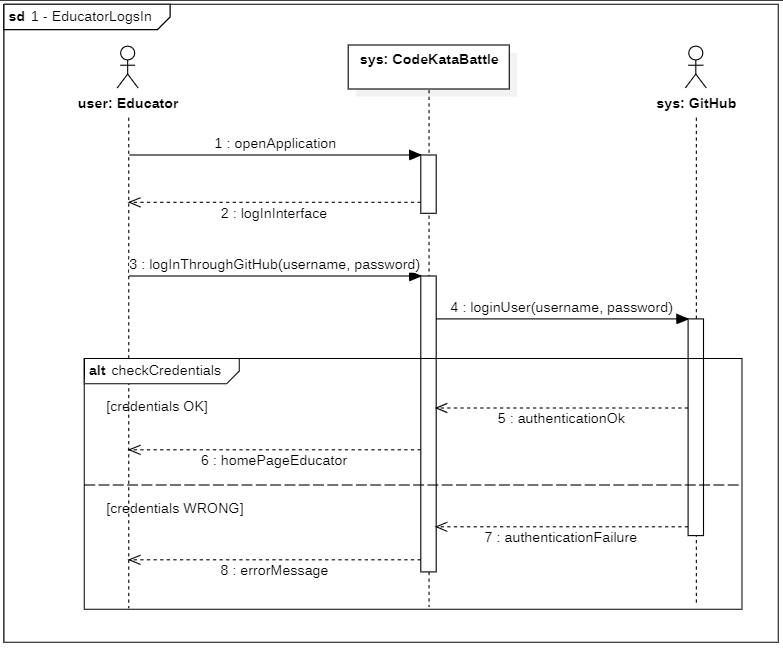
\includegraphics{1EducatorLogsIn}
\end{center}
\end{minipage}

\begin{minipage}{\textwidth}
\textbf{2 - StudentLogsIn}
\begin{center}
	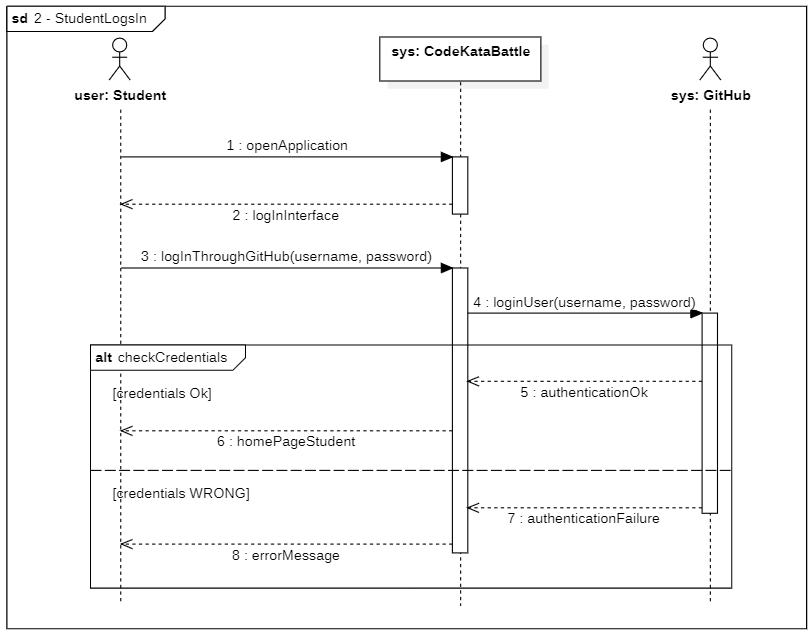
\includegraphics{2StudentLogsIn}
\end{center}
\end{minipage}

\begin{minipage}{\textwidth}
	\textbf{3 - CreateTournament}
	\begin{center}
		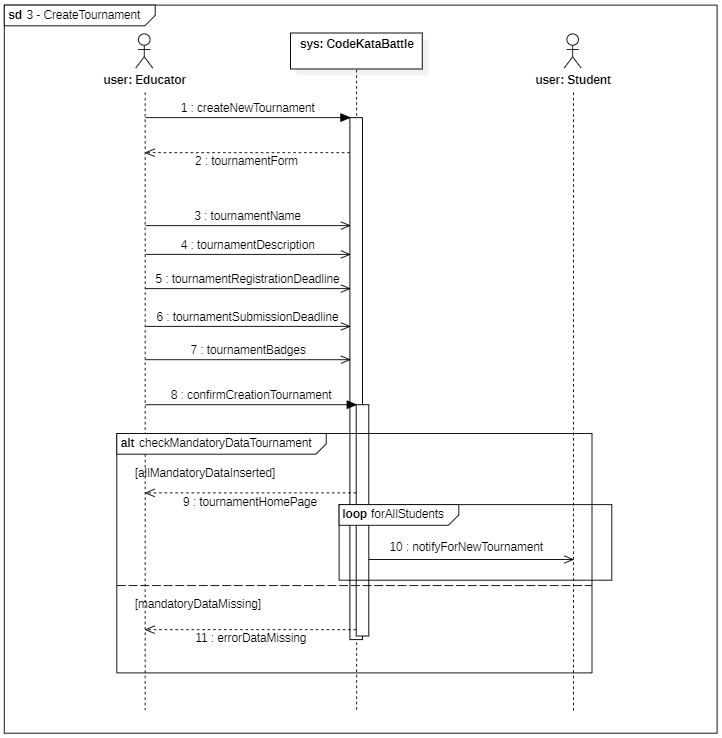
\includegraphics{3CreateTournament}
	\end{center}
\end{minipage}

\begin{minipage}{\textwidth}
	\textbf{4 - CreateBattle}
	\begin{center}
		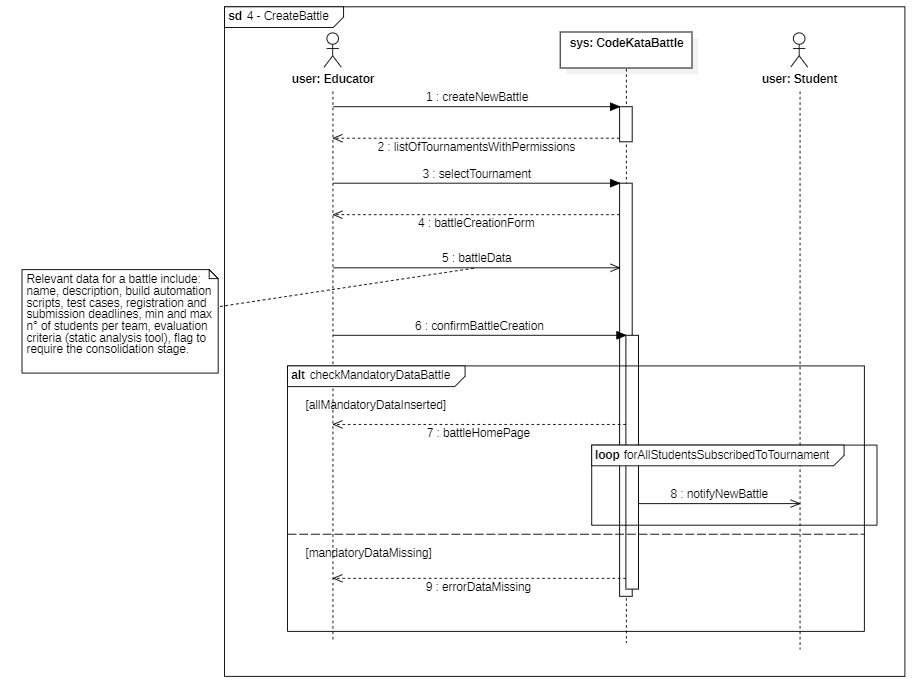
\includegraphics[scale=0.8]{4CreateBattle}
	\end{center}
\end{minipage}

\begin{minipage}{\textwidth}
	\textbf{5 - GrantPermissions}
	\begin{center}
		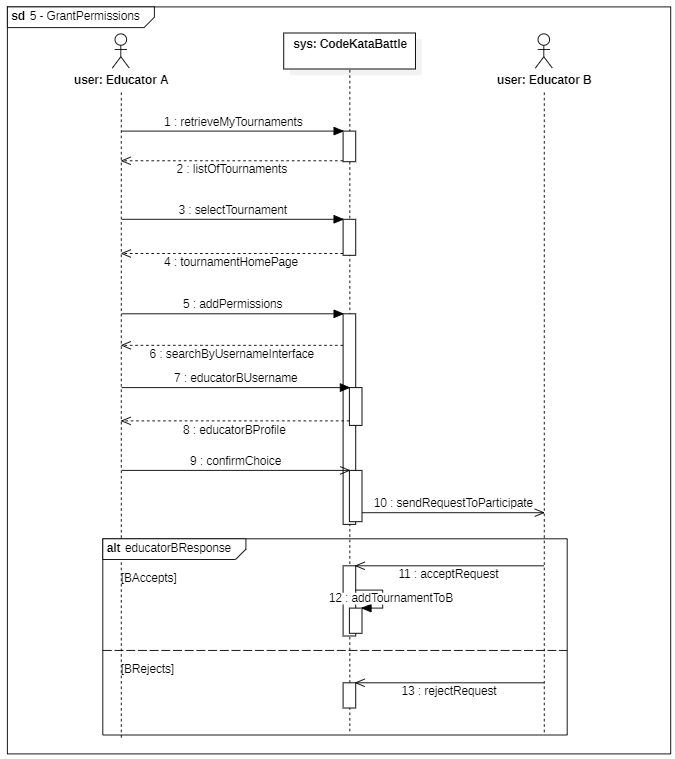
\includegraphics{5GrantPermissions}
	\end{center}
\end{minipage}

\begin{minipage}{\textwidth}
	\textbf{6 - SubscribeToTournament}
	\begin{center}
		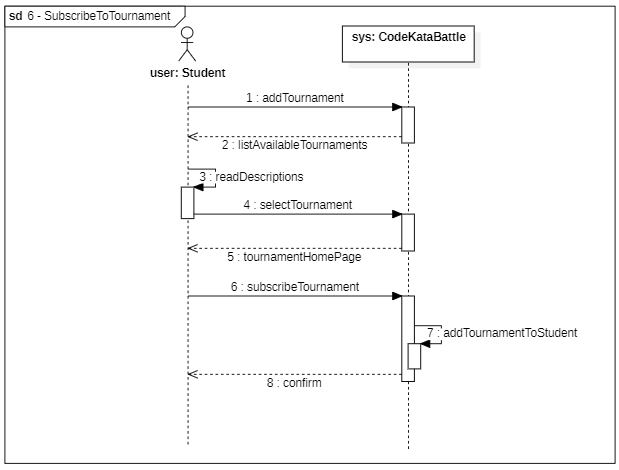
\includegraphics{6SubscribeToTournament}
	\end{center}
\end{minipage}

\begin{minipage}{\textwidth}
	\textbf{7 - JoinBattleAlone}
	\begin{center}
		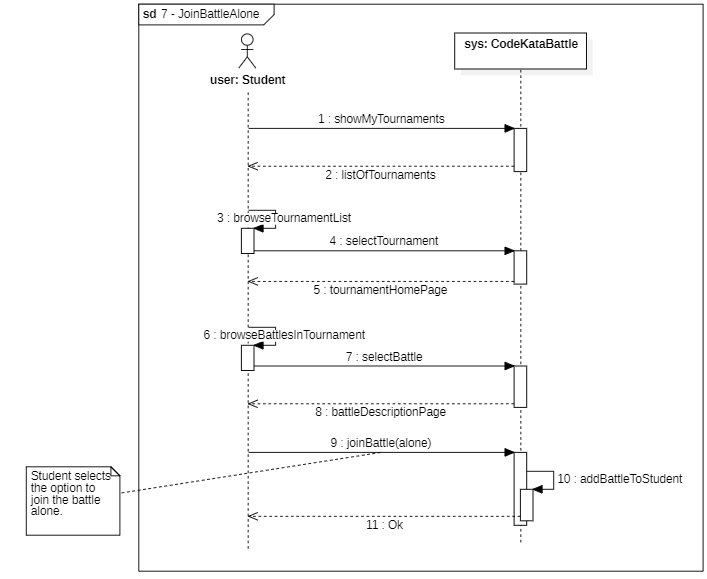
\includegraphics{7JoinBattleAlone}
	\end{center}
\end{minipage}

\begin{minipage}{\textwidth}
	\textbf{8 - JoinBattleAsTeam}
	\begin{center}
		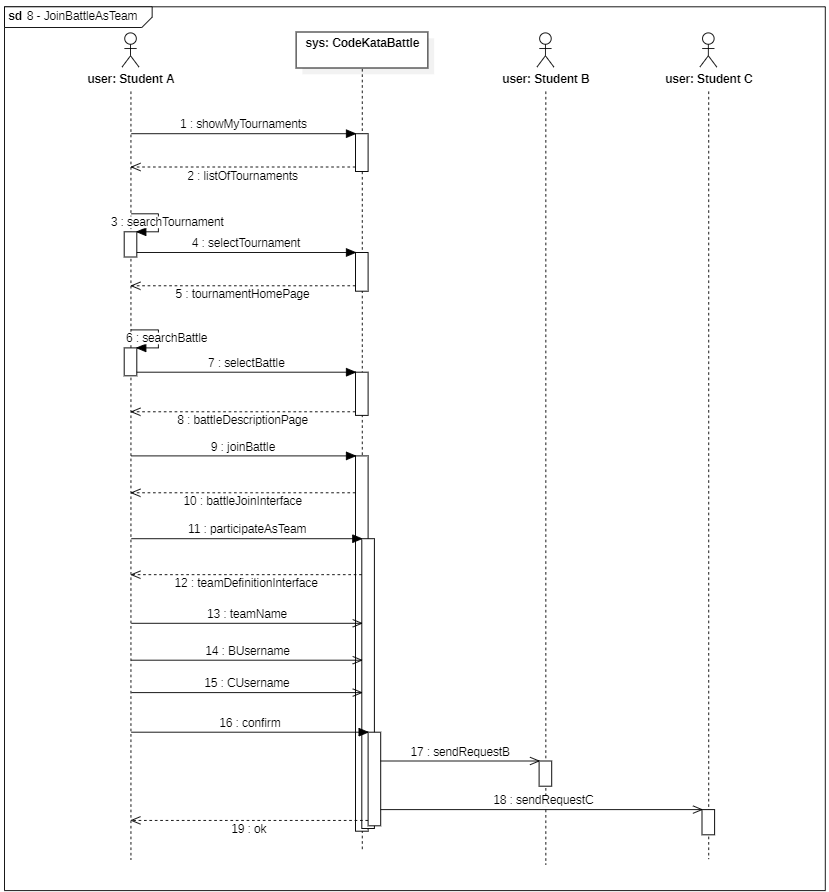
\includegraphics{8JoinBattleAsTeam}
	\end{center}
\end{minipage}

\begin{minipage}{\textwidth}
	\textbf{9 - CreateGitHubRepository}
	\begin{center}
		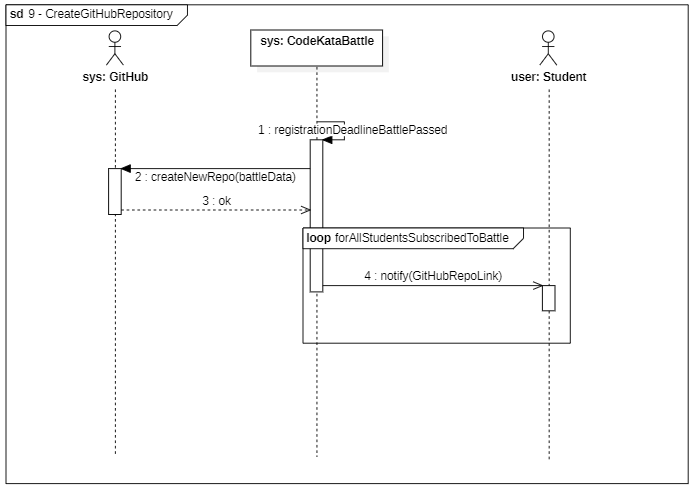
\includegraphics{9CreateGitHubRepository}
	\end{center}
\end{minipage}

\begin{minipage}{\textwidth}
	\textbf{10 - PushSolutionGitHub}
	\begin{center}
		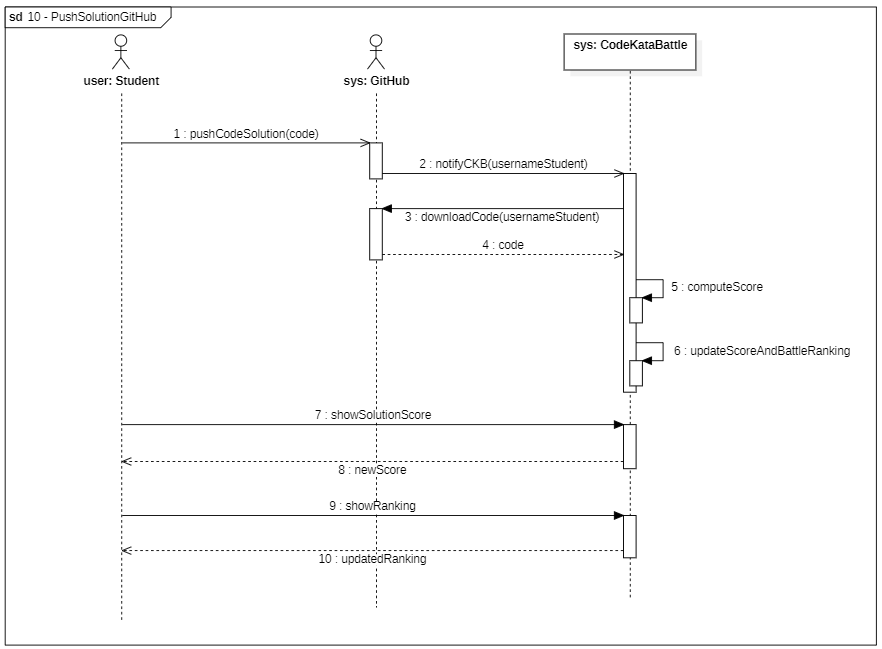
\includegraphics[scale=0.8]{10PushSolutionGitHub}
	\end{center}
\end{minipage}

\begin{minipage}{\textwidth}
	\textbf{11 - CalculateScore}
	\begin{center}
		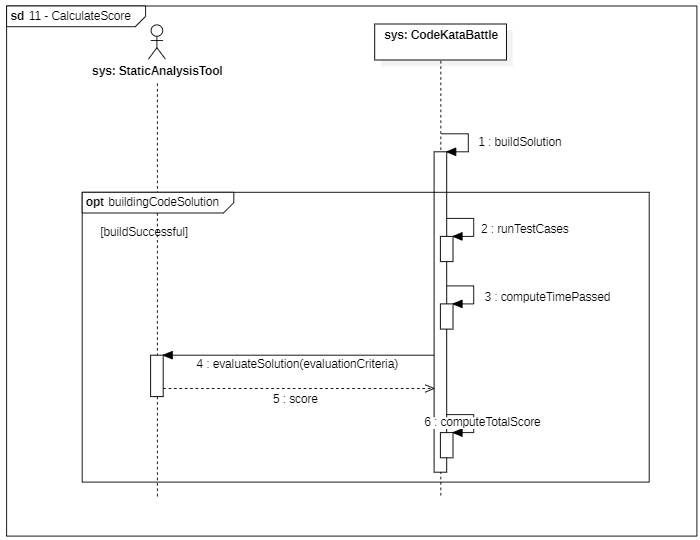
\includegraphics{11CalculateScore}
	\end{center}
\end{minipage}

\begin{minipage}{\textwidth}
	\textbf{12 - EvaluateSolutions}
	\begin{center}
		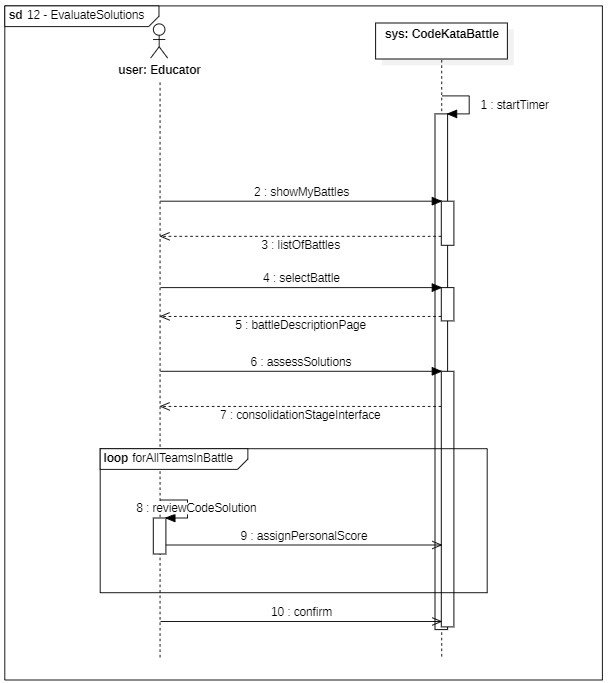
\includegraphics{12EvaluateSolutions}
	\end{center}
\end{minipage}

\begin{minipage}{\textwidth}
	\textbf{13 - TerminateBattle}
	\begin{center}
		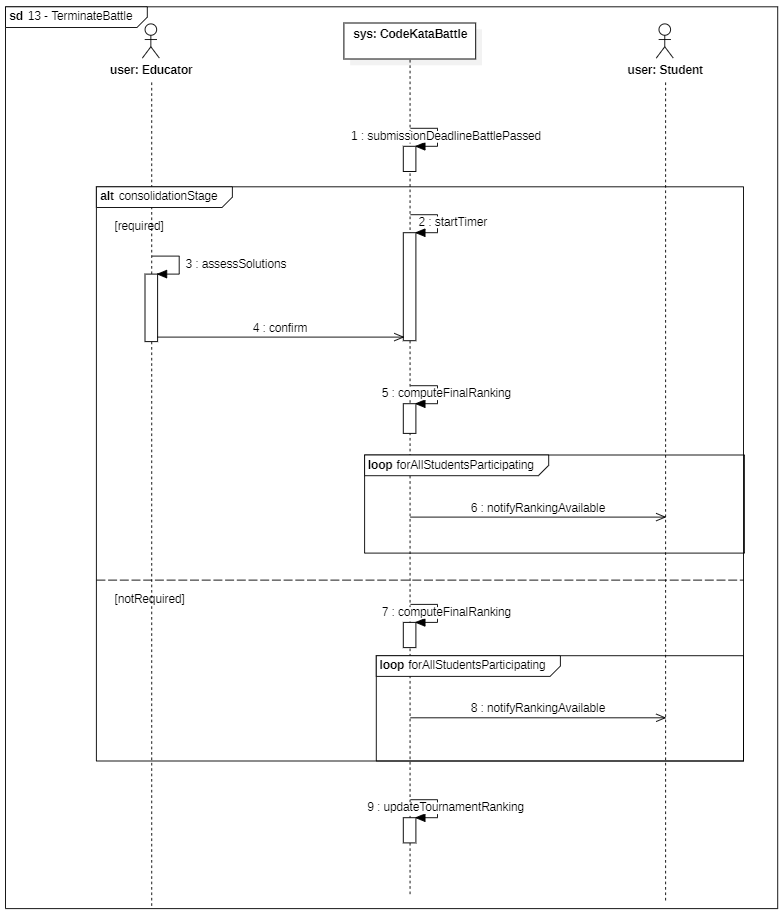
\includegraphics{13TerminateBattle}
	\end{center}
\end{minipage}

\begin{minipage}{\textwidth}
	\textbf{14 - CloseTournament}
	\begin{center}
		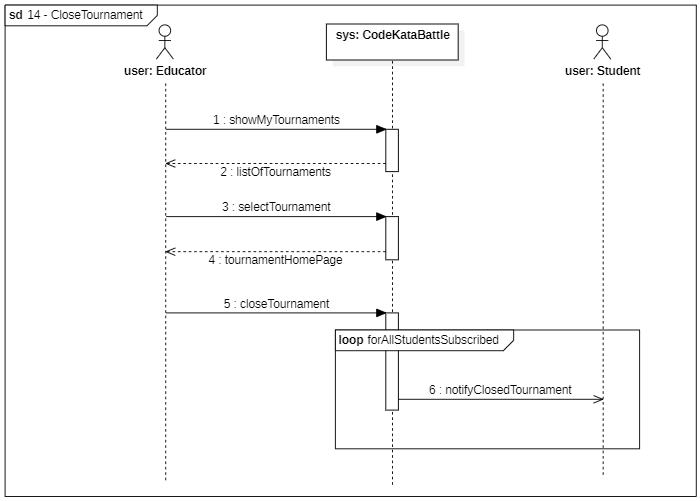
\includegraphics{14CloseTournament}
	\end{center}
\end{minipage}

\begin{minipage}{\textwidth}
	\textbf{15 - OpenTournamentRanking}
	\begin{center}
		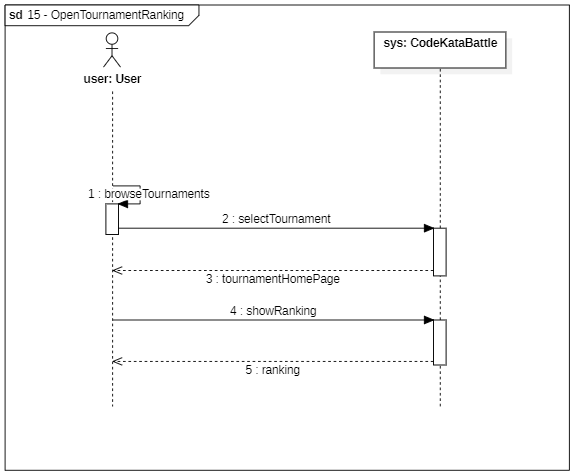
\includegraphics{15OpenTournamentRanking}
	\end{center}
\end{minipage}

\begin{minipage}{\textwidth}
	\textbf{16 - OpenBattleRanking}
	\begin{center}
		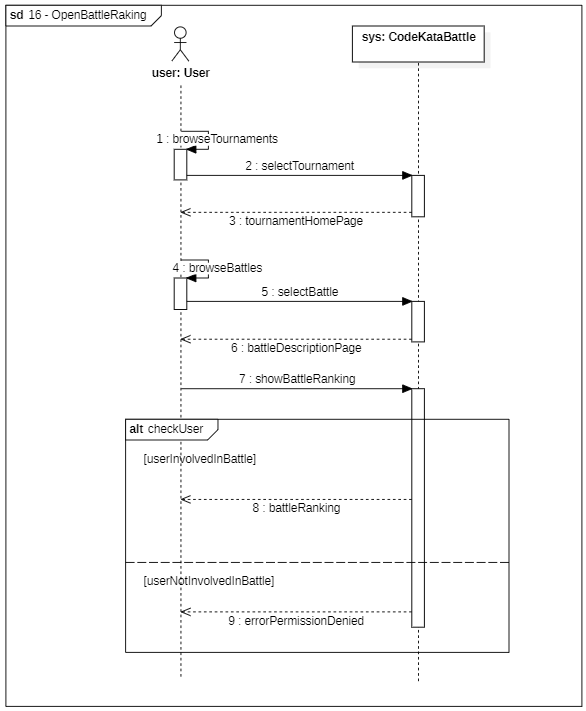
\includegraphics{16OpenBattleRanking}
	\end{center}
\end{minipage}

\begin{minipage}{\textwidth}
	\textbf{17 - ShowProfileAndBadges}
	\begin{center}
		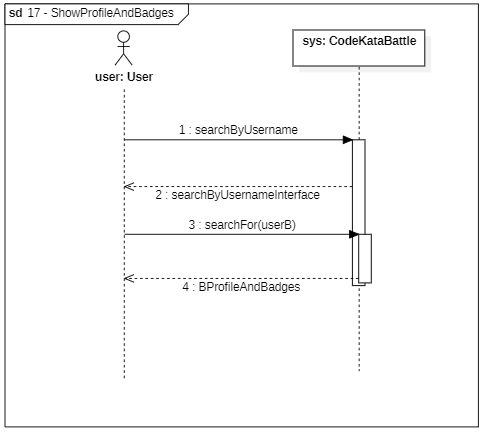
\includegraphics{17ShowProfileAndBadges}
	\end{center}
\end{minipage}
\subsubsection{Requirements Mapping}

\hspace{0.5cm}

\begin{tabular}{|p{8cm}|p{8cm}|}
\hline
\multicolumn{2}{|p{16cm}|}{[G1] The system allows students to practice and improve their coding skills by developing solutions to code kata battles.}\\
\hline
 & Qui\\
Ciaoooooooooo & ciaooooo \\
\hline
\end{tabular}

\vspace{1cm}

\begin{tabular}{|p{8cm}|p{8cm}|}
\hline
\multicolumn{2}{|p{16cm}|}{[G2] The system provides to educators a platform to publish code kata battles and easily manage tournaments and battles for students.}\\
\hline
Plutooooooooooo & Qui\\
Ciaoooooooooo & ciaooooo \\
\hline
\end{tabular}

\vspace{1cm}

\begin{tabular}{|p{8cm}|p{8cm}|}
\hline
\multicolumn{2}{|p{16cm}|}{[G3] The system makes the task of coding battles' solutions as fun as possible, introducing elements like competitiveness, rankings, teamwork and badges (or rewards).}\\
\hline
Plutooooooooooo & Qui\\
Ciaoooooooooo & ciaooooo \\
\hline
\end{tabular}
\newpage
\subsection{Performance Requirements}
The \textit{Code Battle} application must deliver efficient performance to meet the demands of students and educators engaging in coding challenges. The system should aim for low latency, ensuring that the time between user interactions and system responses does not exceed a few seconds under normal internet conditions, but it not a strict condition due to the nature of the application. It is acknowledged that users with slower internet connections may experience increased response times due to external factors beyond the system's control. The application should include mechanisms to detect and handle such situations effectively, but it is not mandatory. 


\subsection{Design Constraints}
\subsubsection{Standard Compliance}
In accordance with data privacy standards, the \app application operates within the framework of the General Data Protection Regulation (GDPR) in order to guarantee the privacy for students and educators data. This regulation governs data protection and privacy for individuals within the European Union (EU) and 
the European Economic Area (EEA). 
The application also adopts international standards for date and time representation.


\subsubsection{Hardware Limitations}
Students and educators hardware requirements are:
\begin{itemize}
    \item Internet connection (2G/3G/4G/5G/Wi-Fi)
    \item iOS/Android smartphone or computer with any modern web browser installed (Chrome, Opera, Firefox, Edge, and others)
\end{itemize}

\subsubsection{Other Constraints}
\newpage
\subsection{Software System Attributes}
\subsubsection{Reliability}
\subsubsection{Availability}
Given that \textit{Code Battle} is not an emergency service, the system can maintain an availability rate less then 99.9 percent. The average time between a fault occurrence and service recovery (MTTR) should be contained at a maximum of 7 days out of 365 per year. This implies that the service could remain highly available still not being completely reliable.


\subsubsection{Security}
As the system stores sensitive personal information about students and educators, security is of great importance. The central database must be fortified with comprehensive security measures to prevent external and internal attacks. Passwords stored in the data store must be encrypted, and in the case of password recovery, clear-text transmission should be avoided. All the channel of communication (e.g. notifications, mails) are assured to be encrypted in relation to the information contained in their messages (e.g. a password recovery is different from a reminder notification). Communication over the internet must utilize encryption to prevent traffic sniffing and spoofing, ensuring privacy and data consistency. 


\subsubsection{Maintainability}
\subsubsection{Portability}
The application must be developed as a web application, so it can be used by smartphones, tablets and computers having modern web browser. In other words, the web application should be compatible with any operating system (e.g., Windows, Mac OS, Linux) that supports a web browser. For this reason it could be developed in a common programming language which guarantees the use of a virtual machine employed in the market (e.g. C, C++, C\# don't seem to be a good choice; instead Java or Python do) 


\newpage